% === Revtex Declaration ===
\documentclass[aps, 10pt, english, twoside, twocolumn, pra, nofootinbib, tightenlines, longbibliography, superscriptaddress]{revtex4-1}

% === All of the Packages I use frequently ===
\usepackage{packages/document_config}
\usepackage{packages/shared}
\usepackage{packages/misc_commands}

\begin{document}
    \title{Edge-Weighted Hypergraph Transversals \& Contextuality}
    \author{Thomas C. Fraser}
    \email{tcfraser@tcfraser.com}
    \affiliation{Perimeter Institute for Theoretical Physics, Waterloo, Ontario, Canada, N2L 2Y5}
    \affiliation{University of Waterloo, Waterloo, Ontario, Canada, N2L 3G1}
    % \author{Elie Wolfe}
    % \affiliation{Perimeter Institute for Theoretical Physics, Waterloo, Ontario, Canada, N2L 2Y5}
    % \email{ewolfe@perimeterinstitute.ca}
    \date{\today}
    \begin{abstract}
        This is the abstract.
    \end{abstract}
    \maketitle
    \tableofcontents

    \section{Introduction}
    \subsection{Applications}

    \section{Marginal Satisfiability}
    \subsection{Definitions}
    To every random variable\footnote{Throughout this document, it is assumed that all random variables are discrete and have finite cardinality.} $v$ there corresponds a prescribed set of \term{outcomes} $\outcomes{v}$ and a set of \term{events over $v$} denoted $\events{v}$ corresponding to the set of all functions of the form $\w : \bc{v} \to \outcomes{v}$. Evidently, $\events{v}$ and $\outcomes{v}$ are isomorphic structures and their distinction can be confounding. There is rarely any harm in referring synonymously to either as outcomes. Nonetheless, a sheaf-theoretic treatment of contextuality \cite{Abramsky_2011} demands the distinction. Specifically for this work, the distinction becomes essential for the exploitation of marginal symmetries in \cref{sec:marginal_symmetries}. As a natural generalization we define the event over a collection of random variables $V = \bc{v_1, \ldots, v_n}$ in a parallel manner:
    \[ \events{V} \defined \bc{\w : V \to \outcomes{V} \mid \forall v \in V, \w\br{v} \in \outcomes{v}} \]
    Furthermore, the \term{domain $\domain{\w}$} of an event $\w$ is the set of random variables it valuates, i.e. if $\w \in \events{V}$ then $\domain{\w} = V$.

    For every $V' \subset V$ and $\w \in \events{V}$, the \term{restriction of $\w$ onto $V'$} (denoted $\restrict{\w}{V'}$) corresponds to the unique event in $\events{V'}$ that agrees with $\w$ for all valuations of variables in $V'$, i.e. $\forall v' \in V': \restrict{\w}{V'}\br{v'} = \w\br{v'}$. Using this notational framework, a probability distribution or simply \term{distribution} $\prob{V}$ is a probability measure on $\events{V}$, assigning to each $\w \in \events{V}$ a real number $\prob{V}\br{\w} \in \bs{0,1}$ such that $\sum_{\w \in \events{V}} \prob{V}\br{\w} = 1$. The set of all distributions over $\events{V}$ is denoted $\probset{V}$. Moreover, given $\prob{V} \in \probset{V}$ and $V' \subset V$, there is an induced distribution $\restrict{\prob{V}}{V'} \in \probset{V'}$ obtained by \textit{marginalizing} $\prob{V}$:
    \[ \restrict{\prob{V}}{V'}\br{\w'} = \sum_{\substack{\w \in \events{V} \\ \restrict{\w}{V'} = \w'}} \prob{V}\br{\w} \eq \label{eq:marginalization_defined} \]
    Presently, the reader is equipped with sufficient notation and terminology to comprehend the \term{marginal (satisfiability) problem}: given a collection of $m$ distributions $\bc{\prob{V_1},\ldots,\prob{V_m}}$, does there exist a distribution $\prob{\jointvar} \in \probset{\jointvar}$ where $\jointvar \defined \bigcup_{i = 1}^{m} V_m$ such that $\forall i : \restrict{\prob{\jointvar}}{V_i} = \prob{V_i}$?

    To facilitate further discussion of this problem, several pieces of nomenclature will be introduced. First, the set $\mscenario = \bc{V_1, \ldots, V_m}$ is called the \term{marginal scenario} while its elements are called the \term{marginal contexts}. The collection of distributions $\prob{\mscenariowrap} \defined \bc{\prob{V_1},\ldots,\prob{V_m}}$\footnote{The subscript $*$ preceding $\mscenariowrap$ is added for clarity; $\prob{\mscenariowrap}$ is \textit{not} a distribution but a set of distributions over $\mscenario$. The $\mscenariowrap$ convention is adopted throughout this report.} is called the \term{marginal model}~\cite{Fritz_2011}\footnote{In~\cite{Abramsky_2011}, $\prob{\mscenariowrap}$ is instead called an \textit{empirical model}.}. The distribution $\prob{\jointvar}$, if it exists, is termed the \term{joint distribution}. Strictly speaking, as defined by~\cite{Fritz_2011}, a marginal scenario forms an \textit{abstract simplicial complex}, meaning it satisfies the supplementary required that all subsets of contexts are also contexts, i.e. $\forall V \in \mscenario : V' \subset V \implies V' \in \mscenario$. Throughout this work, we exclusively consider (without loss of generality) \textit{maximal} marginal scenarios, restricting our focus to the contexts which are contained in no others. Finally, a marginal model $\prob{\mscenariowrap}$ is said to be \term{contextual}, and will be denoted $\prob{\mscenariowrap} \in \s C \subseteq \probset{\mscenariowrap}$ if it does not admit a joint distribution and \term{non-contextual} otherwise ($\prob{\mscenariowrap} \not \in \s C$). Equipped with additional terminology and notation, the marginal problem now reads: given $\prob{\mscenariowrap}$, is $\prob{\mscenariowrap} \in \s C$ or not?

    \subsection{Linearity}
    An essential feature of the marginal problem is linearity; the marginalization of $\prob{\jointvar}$ onto the marginal contexts $\bc{\restrict{\prob{\jointvar}}{V} \mid V \in \mscenario}$ is a linear transformation, requiring only the summations pursuant to \cref{eq:marginalization_defined}. Consequently, it is advantageous to consider the statement of the marginal problem as a matrix multiplication. To this end, for each marginal scenario $\mscenario$ we define a bitwise matrix $\incidence$ called the \term{incidence matrix} which implements this mapping. The columns of $\incidence$ are indexed by \textit{joint events} $j \in \events{\jointvar}$ and the rows are indexed by \textit{marginal events} $m \in \events{V}$ for some $V \in \mscenario$. By deliberate abuse of notation, we will denote the set of all marginal events as $\events{\mscenariowrap}$ and is defined as the following disjoint union:
    \[ \events{\mscenariowrap} \defined \coprod_{V \in \mscenario} \events{V} \]
    The $\abs{\events{\mscenariowrap}}\times\abs{\events{\jointvar}}$ incidence matrix $\incidence$ is then defined element-wise for $m \in \events{\mscenariowrap}$ and $j \in \events{\jointvar}$:
    \[ \incidence^{m}_{j} = \begin{cases}
        1 & \restrict{j}{\domain{m}} = m\\
        0 & \text{otherwise}
    \end{cases} \]
    Conceptually, the entries of this matrix are populated with ones whenever the marginal event (row) $m$ is the restriction of some joint event (column) $j$. For a given marginal scenario $\mscenario$, $\incidence$ represents the tuple of restriction maps $\incidence : \events{\jointvar} \to \prod_{V \in \mscenario} \events{V} :: j \mapsto \bc{\restrict{j}{V} \mid V \in \mscenario}$~\cite{Abramsky_2011}.

    To illustrate this concretely, consider the following example. Let $\jointvar$ be $3$ binary variables $\bc{a,b,c}$ and $\mscenario$ be the marginal scenario $\mscenario = \bc{\bc{a,b}, \bc{b,c}, \bc{a,c}}$. The incidence matrix for $\mscenario$ becomes:
    \begin{equation}
        \resizebox{1.0\hsize}{!}{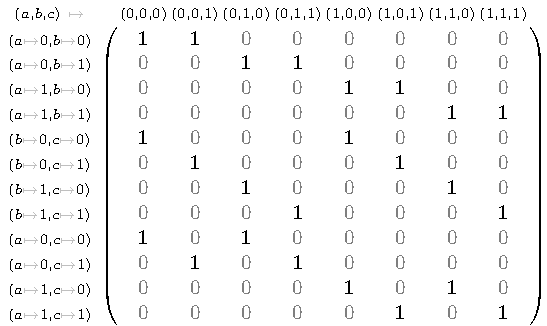
\includegraphics{figures/incidence_matrix_1_example/figure.pdf}}
        \label{eq:incidence_example}
    \end{equation}

    In addition, for any joint distribution $\prob{\jointvar} \in \probset{\jointvar}$ we associate a joint distribution \textit{vector} $\prob{\jointvar}$ (identically denoted) indexed by $j \in \events{\jointvar}$, i.e. $\prob{\jointvar}^{j} \defined \prob{\jointvar}\br{j}$. Analogously, for each marginal model $\prob{\mscenariowrap} \in \probset{\mscenariowrap}$ there is an associated marginal distribution \textit{vector} $\prob{\mscenariowrap}$ indexed by $m \in \events{\mscenariowrap}$ such that $\prob{\mscenariowrap}^{m} \defined \prob{\domain{m}}\br{m}$. Using these vectors, the marginal problem becomes the following linear program: given a marginal distribution vector $\prob{\mscenariowrap}$, does there exist a joint distribution vector $\prob{\jointvar} \succeq 0$ such that \cref{eq:incidence_marginal_problem} holds?
    \[ \prob{\mscenariowrap} = \incidence \cdot \prob{\jointvar} \iff \prob{\mscenariowrap}^{m} = \sum_{j \in \events{\jointvar}} \incidence^{m}_{j} \prob{\jointvar}^{j} \eq \label{eq:incidence_marginal_problem} \]

    \subsection{Marginal Polytopes}

    \subsection{Logical Contextuality}
    Let $a \in \events{\mscenariowrap}$ be \textit{any} marginal event and $C = \bc{c_1, \ldots, c_n} \subseteq \events{\mscenariowrap}$ be a subset of marginal events such that the following logical implication holds for \textit{all} marginal models $\prob{\mscenariowrap} \in \probset{\mscenariowrap}$:
    \[ a \implies c_1 \vee \cdots \vee c_n = \bigvee_{c \in C} c \eq \label{eq:hardy_logical_implication} \]
    Which can be dictated: \textit{whenever the event $a$ occurs, at least one event in $C$ occurs.} In accordance with the logical form of \cref{eq:hardy_logical_implication}, $a$ will be referred to as the \term{antecedent} and $C$ as the \term{consequent set}. To clarify, a marginal model $\prob{\mscenariowrap} \in \probset{\mscenariowrap}$ satisfies \cref{eq:hardy_logical_implication} if there always at least one $c \in C$ that is \textit{possible} ($\prob{\mscenariowrap}^{c} > 0$) whenever $a$ is possible. A marginal model violates \cref{eq:hardy_logical_implication} whenever \textit{none} of events in $c$ are possible while $a$ remains possible. Marginal models that violate logical statements such as \cref{eq:hardy_logical_implication} are known as \term{Hardy Paradoxes}~\cite{Inflation,Mansfield_2012,Mancinska_2014}. Motivated by a greater sense of robustness compared to possibilistic constraints, the concept of witnessing quantum contextuality on a logical level has be analyzed thoroughly for decades~\cite{Abramsky_2012,Greenberger_1990}.

    \section{An Observation}
    \subsection{An Antecedent Hierarchy}
    \subsection{The Antecedent Hypergraph}
    Given an antecedent multi-set $\multiset$ where $\multiset \preceq 0$, we identify the \term{inhibiting set} of joint events $\inhibit{\multiset} \subseteq \events{\jointvar}$ preventing $\multiset \cdot \incidence$ from being positive semi-definite:
    \[ \inhibit{\multiset} \defined \bc{j \in \events{\jointvar} \mid \sum_{m \in \events{\mscenariowrap}} \multiset^{m} \incidence^{j}_{m} < 0} \]
    The inhibiting set $\inhibit{\multiset}$ of $\multiset$ completely characterizes the \term{antecedent hypergraph} $\hypergraph\br{\multiset}$ whose edges $\edges_{j}$ are indexed by the inhibiting events $j \in \inhibit{\multiset}$. Each edge $\edges_{j} \subseteq \events{\mscenariowrap}$ corresponds to the set of the marginal events $m \in \events{\mscenariowrap}$ which are restrictions of $j$. Specifically,
    \begin{gather*}
        \hypergraph\br{\multiset} \defined \bc{\edges_j \mid j \in \inhibit{\multiset}} \\
        \edges_{j} \defined \bc{m \in \events{\mscenariowrap} \mid m = \restrict{j}{\domain{m}}, \multiset^{m} = 0}
    \end{gather*}

    \subsection{Irreducibility}
    \subsection{Marginal Symmetries}
    \label{sec:marginal_symmetries}
    \subsection{Curated Inequalities}
    \subsection{Targeted Searches}
    \subsection{Relaxations}

    \section{Edge-Weighted Hypergraph Transversals}
    \subsection{Preliminaries}
    \begin{center}
        \begin{figure}
            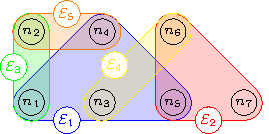
\includegraphics[width=\linewidth]{figures/hypergraph_diagram_1_standalone/figure.pdf}
            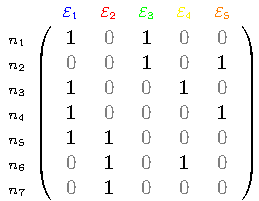
\includegraphics[width=0.8\linewidth]{figures/hypergraph_matrix_1_standalone/figure.pdf}
            \caption{Dual-representations of a hypergraph $\hypergraph = \bc{\edges_1,\edges_2,\edges_3,\edges_4,\edges_5}$.}
        \end{figure}
    \end{center}
    \subsection{Hypergraph Transversals}
    \subsection{Adding Weights}

    \section{Conclusions}
    \section*{Acknowledgments}

    \setlength{\bibsep}{3pt plus 3pt minus 2pt}
    \bibliographystyle{apsrev4-1}
    \nocite{apsrev41Control}
    \bibliography{references}

\end{document}
